% Chapter 4

\chapter{Desarrollo}
\label{capitulo4}

\section{Preperaciones del Ambiente de Desarrollo}

\subsection{Sistema Base de Desarrollo}

\begin{figure}
	\begin{center}
    	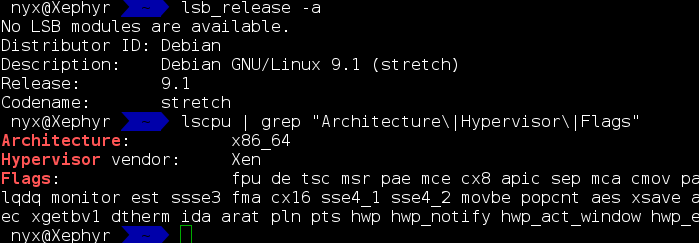
\includegraphics[width=0.75\textwidth]{Figures/sistema-base.png}
    \end{center}
  	\caption{Información del Sistema Base.}
    \label{sistema-base}
\end{figure}

Como se presenta en la figura \ref{sistema-base}, el sistema base para el desarrollo de este trabajo de titulacion utiliza Xen instalado con Debian Stretch (9.1)\footnote{Como el sistema de Dom0} instalado en un LVM con el nombre del grupo de volumenes ''Xephyr-VG''. Originalmente se tenia planificado trabajar con Debian Jessie (8.x) debido que eso fue la version estable al momento de instalacion pero despues se opto por una actualizacion a la version beta de Debian en aquello momento (Debian Stretch). En resumen los pasos realizados fueron:
\lstset{language=Bash}
\begin{enumerate}
	\item Instalacion Limpia de Debian 8 con un LVM.
    	\begin{description}
    		\item[Volumen Fisico:] /dev/sda8 310g 
            \item[Grupo de Volumenes:] Xephyr-VG 310g
            \item[Volumenes Logicos:] Originalmente 4 (se agrega 2 por cada nueva maquina virtual -- uno para su disco y otro para su area de intercambio).
            \begin{description}
            	\item[Xephyr-Dom0] Xephyr-VG 30g
                \item[Xephyr-IMG-Repo] Xephyr-VG 20g
                \item[Xephyr-ISO-Repo] Xephyr-VG 20g
                \item[Xephyr-Swap] Xephyr-VG 4g
            \end{description}
    	\end{description}
    \item Actualizar Instalacion de Debian 8.
    	\begin{lstlisting}
	apt update
	apt upgrade
	apt dist-upgrade
	reboot
        \end{lstlisting}
    \item Actualizar Debian 8 a Debian 9.
        \begin{lstlisting}
	sed -i 's/jessie/stretch/g' /etc/apt/sources.list
	apt update
	apt upgrade
	reboot
        \end{lstlisting}
    \item Instalacion de Herramientas de Trabajo
        \begin{lstlisting}
	apt install tmux vim zsh
        \end{lstlisting}
    \item Instalacion y Configuracion de Hipervisor Xen
		\begin{lstlisting}
	apt install xen-hypervisor
	dpkg-divert --divert /etc/grub.d/08_linux_xen \
		--rename /etc/grub.d/20_linux_xen
	update-grub
	cat > /etc/network/interfaces.d/xenbr << EOF

	auto xenbr0
	iface xenbr0 inet static
		address 10.10.10.1
		netmask 255.255.255.0
		bridge_ports wlan0

	#other possibly useful options in a
	#	virtualized environment
		#bridge_stp off		# disable
		#		Spanning Tree Protocol
		#bridge_waitport 0	# no delay
		#		before a port becomes
		#		available
		#bridge_fd 0		# no forwarding
		#		delay

	## configure a (separate) bridge for
	#	the DomUs without giving Dom0 an
	#	IP on it
	#auto xenbr1
	#iface xenbr1 inet manual
	#   bridge_ports eth1

	EOF

	reboot
		\end{lstlisting}
	\item Instalacion de Herramientas de Xen
		\begin{lstlisting}
	apt install xen-tools xen-utils
		\end{lstlisting}
    \item Instalacion de Herramientas de Desarrollo para Python 3
    	\begin{lstlisting}
	apt install python3 python3-virtualenv python3-pip
    	\end{lstlisting}
    \item Instalacion de Servidores
    	\begin{lstlisting}
	apt install nginx-full postgresql mongodb\
    		redis-server
    	\end{lstlisting}
    \item Instalacion de IDEs en /opt. Se descargaron los respetivos .tar\textit{.xx} y se los descomprimieron en /opt con un comando similar al siguiente:
    	\begin{lstlisting}
	tar -axvf nombre.tar.xx -C\
    		/opt/ruta/raiz/donde/descomprimir
    	\end{lstlisting}
    \begin{enumerate}
    	\item PyCharm (Community o Professional Edition\footnote{Se ocupo una version Professional, en parte por su buen suporte para desarrollo en Django) con una licencia estudiantil que actualmente es gratis de solicitar y renovar año tras año con un correo institucional})
        \item DBeaver (Community o Enterprise Edition\footnote{Historicamente siempre han sido gratis ambas versiones con la diferencia siendo que Enterprise Edition no es completamente software libre a diferencia de su version libre, pero el mismo agrega suporte para bases de datos no relacionales. Se ocupo la version Enterprise, entre los ultimos ofertas gratis antes de que se convierte en un producto de pago, por este mismo motivo de requerir suporte para bases de datos NoSQL como MongoDB y Redis.})
    \end{enumerate}
\end{enumerate}

Estos pasos de instalacion se basaron en la guia de instalacion de Xen publicado en el wiki del proyecto de Debian \citep{Debian-Wiki-Xen}.

Para dar connexiones hace el exterior a las maquinas virtuales, se necesita activar una regla NAT en el cortafuego IPTables:

\begin{lstlisting}
	iptables -t nat -A POSTROUTING -o wlan0\
    		-j MASQUERADE
\end{lstlisting}

\subsection{Ambiente Virtual de LMS (Moodle)}
\label{instalacion-moodle}

Para el ambiente de Moodle (LMS contra el cual se ha llevado el desarrollo), se crea una maquina virtual de Debian Stretch (9) con 1 GiB de RAM, 1 CPU virtual, 6 GiB de disco, 512 MiB de intercambio y una direccion IP fija de 10.10.10.10. Los resultados del mismo commando se puede ver en la figura \ref{vm-moodle}.
\begin{lstlisting}
	xen-create-image --hostname=debian-moodle\
    		--ip=10.10.10.10 --netmask=255.255.255.0\
        	--gateway=10.10.10.1 --memory=1024mb\
        	--vcpus=1 --lvm=Xephyr-VG --pygrub\
        	--dist=stretch --force --size=6144mb\
        	--swap=512mb
\end{lstlisting}

\begin{figure}
	\begin{center}
    	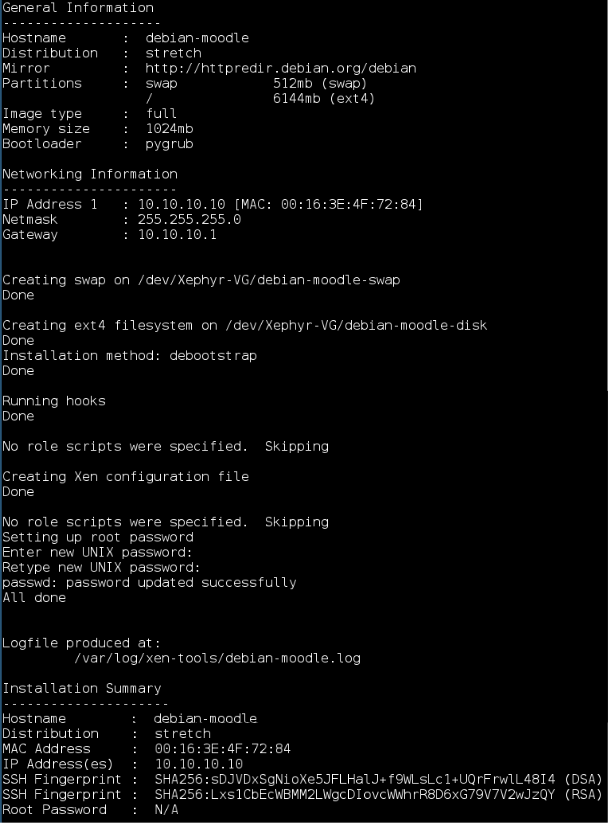
\includegraphics[width=0.75\textwidth]{Figures/crear-moodle.png}
    \end{center}
  	\caption{Crear maquina virtual para Moodle.}
    \label{vm-moodle}
\end{figure}

Se renombró el archivo de configuracion de la maquina virtual generado en el paso anterior para temas de consistencia.

\begin{lstlisting}
	mv /etc/xen/debian-moodle.cfg\
    		/etc/xen/domU-debian-moodle.cfg
\end{lstlisting}

Un bug de Xen-Tools causa que no se instala correctamente un nucleo de Linux en la maquina virtual y por lo tanto es necesario entrar al mismo con un Chroot y instalar los paquetes faltantes (y hacer las adecuadas configuraciones  para permitir su aranque independiente de ayuda externa).

\begin{lstlisting}
	mount /dev/Xephyr-VG/debian-moodle-disk /mnt
	mount -o bind /proc /mnt/proc
	mount -o bind /sys /mnt/sys
	mount -o bind /dev /mnt/dev
	cp /etc/resolv.conf /mnt/etc/resolv.conf
	chroot /mnt /bin/bash
	apt install linux-image-amd64
	vim.tiny /boot/grub/menu.lst
	# Revisar que los archivos referenciados existen
	#		de verdad por ejemplo:
	# Replace initrd.img- con initrd.img
    # guarda y sale
	exit
	umount /mnt/proc            
	umount /mnt/sys 
	umount /mnt/dev 
	umount /mnt	
\end{lstlisting}

Para levantar la maquina virtual:

\begin{lstlisting}
	xl create /etc/xen/domU-debian-moodle.cfg -c
\end{lstlisting}

Se debe selecionar la tercera opcion (Default Kernel).

Se puede dar una revision a la configuracion de red para asegurarse de que esta correcto:

\begin{lstlisting}
	vim.tiny /etc/network/interfaces
\end{lstlisting}

Debe contener:

\begin{lstlisting}
auto eth0
iface eth0 inet static
 address 10.10.10.10
 gateway 10.10.10.1
 netmask 255.255.255.0
\end{lstlisting}

En el presente caso, Xen-Tools logró configurar esta parte de forma correcta.

A continuacion se procede con la instalacion de Moodle:

\begin{lstlisting}
# actualiza el sistema
apt update
apt upgrade

# instala dependencias
apt install apache2 php7.0 mysql-server php7.0-mysql
apt install libapache2-mod-php7.0 php7.0-gd php7.0-curl
apt install php-xml php-zip php-mbstring php-soap
apt install php7.0-xmlrpc php7.0-intl
vim.tiny /etc/php/7.0/apache2/php.ini

# agrega:
extension=mysql.so 
extension=gd.so

# edita:

memory_limit = 40M
# dejado con el valor por defecto de 128M

post_max_size = 80M
upload_max_filesize = 80M

# guarda y sale

# reinicia apache para coger los cambios
systemctl restart apache2

\end{lstlisting}

A continuacion se configura la base de datos:

\begin{lstlisting}

# clave de root es root
mysqladmin -u root password "root"

# logear como root
mysql -u root -p

# crear base de datos y hacer que ocupa UTF-8
mysql> CREATE DATABASE moodle;
mysql> ALTER DATABASE moodle charset=utf8;
mysql> exit;

## No se implemento ##
# Moodle queja de UTF8

# Se podria arreglar
# (antes de instalar Moodle)
# con:

mysql -u root -p

mysql> ALTER DATABASE moodle charset=utf8mb4;
mysql> exit;
######################

systemctl restart mysql

\end{lstlisting}

Se realiza la instalacion de la ultima version de Moodle (3.3 con sus respectivos patches de fallas desde que el mismo salio):

\begin{lstlisting}

# descargar
wget https://download.moodle.org/download.php/direct/stable33/moodle-latest-33.tgz

# descomprimir
tar -zxvf moodle-latest-33.tgz

# meter en ubicacion para apache
mv moodle /var/www

# ir a ubicacion para apache
cd /var/www

# crear ubicacion para datos
mkdir moodledata

# arreglar permisos
chown -R www-data:www-data moodle
chown -R www-data:www-data moodledata
chmod -R 755 moodle
chmod -R 755 moodledata

# modificar configuracion de apache
vim.tiny /etc/apache2/sites-available/000-default.conf

# editar
DocumentRoot "/var/www/moodle"

# guardar y salir

# reiniciar apache para aplicar los cambios
systemctl restart apache2

\end{lstlisting}

Arreglar la base de datos para que acepte conexiones desde Moodle:

\begin{lstlisting}

mysql -u root -p

GRANT ALL PRIVILEGES on *.* to
	'root'@'localhost' IDENTIFIED BY 'root';
GRANT ALL PRIVILEGES on *.* to
	'root'@'localhost' IDENTIFIED BY 'root';
FLUSH PRIVILEGES;
exit;

\end{lstlisting}

Para seguir con la instalacion se abre un navegador con la direccion \url{http://10.10.10.10/} para seguir las instrucciones que se le lleve por toda la configuracion inicial del Moodle.

Al final se agrege un trabajo de cron para ayudar con los tareas periodicas que Moodle requiere para su mantemiento continuo:

\begin{lstlisting}

crontab -u www-data -e
# add line:
*/10 * * * * /usr/bin/php
		/var/www/moodle/admin/cli/cron.php
        		>/dev/null

\end{lstlisting}

Estos pasos fueron adaptados de la guia oficial del proyecto de Moodle para instalacion en Debian \citep{MOODLE-Install-Debian}.

Ahora que todo esta funcionando se recomienda editar /boot/grub/menu.lst para comentar las entradas del pyGrub que son defectuosas (los primeros dos) para que se puede levantar la maquina virtual sin intervencion humana.

\subsection{Servidor de Git (GitLab CE)}
Para crear el servidor de Git con GitLab Community Edition, se va a empezar con las mismas piezas del servidor del LMS/Moodle, es decir una maquina virtual de Debian 9. El mismo se crea como una maquina virtual de Debian Stretch (9) con 1 GiB de RAM, 1 CPU virtual, 6 GiB de disco, 512 MiB de intercambio y una direccion IP fija de 10.10.10.11.
\begin{lstlisting}
	xen-create-image --hostname=debian-gitlab\
    		--ip=10.10.10.11 --netmask=255.255.255.0\
        	--gateway=10.10.10.1 --memory=1024mb\
        	--vcpus=1 --lvm=Xephyr-VG --pygrub\
        	--dist=stretch --force --size=6144mb\
        	--swap=512mb
\end{lstlisting}

Se renombró el archivo de configuracion de la maquina virtual generado en el paso anterior para temas de consistencia.

\begin{lstlisting}
	mv /etc/xen/debian-gitlab.cfg\
    		/etc/xen/domU-debian-gitlab.cfg
\end{lstlisting}

Un bug de Xen-Tools causa que no se instala correctamente un nucleo de Linux en la maquina virtual y por lo tanto es necesario entrar al mismo con un Chroot y instalar los paquetes faltantes (y hacer las adecuadas configuraciones  para permitir su aranque independiente de ayuda externa).

\begin{lstlisting}
	mount /dev/Xephyr-VG/debian-gitlab-disk /mnt
	mount -o bind /proc /mnt/proc
	mount -o bind /sys /mnt/sys
	mount -o bind /dev /mnt/dev
	cp /etc/resolv.conf /mnt/etc/resolv.conf
	chroot /mnt /bin/bash
	apt install linux-image-amd64
	vim.tiny /boot/grub/menu.lst
	# Revisar que los archivos referenciados existen
	#		de verdad por ejemplo:
	# Replace initrd.img- con initrd.img
    # guarda y sale
	exit
	umount /mnt/proc            
	umount /mnt/sys 
	umount /mnt/dev 
	umount /mnt	
\end{lstlisting}

Para levantar la maquina virtual:

\begin{lstlisting}
	xl create /etc/xen/domU-debian-gitlab.cfg -c
\end{lstlisting}

Se debe selecionar la tercera opcion (Default Kernel).

Se puede dar una revision a la configuracion de red para asegurarse de que esta correcto:

\begin{lstlisting}
	vim.tiny /etc/network/interfaces
\end{lstlisting}

Debe contener:

\begin{lstlisting}
auto eth0
iface eth0 inet static
 address 10.10.10.11
 gateway 10.10.10.1
 netmask 255.255.255.0
\end{lstlisting}

En el presente caso, Xen-Tools logró configurar esta parte de forma correcta.

A continuacion se procede con la instalacion de Gitlab:

\begin{lstlisting}
# actualiza el sistema
apt update
apt upgrade

# Apartir del Debian 9, Gitlab CE esta ofrecido
#    en los repositorios oficiales:
apt install gitlab

# Arreglar problema con API
vim.tiny /usr/share/gitlab-shell/config.yml
# cambiar gitlab_url a "http://10.10.10.11/"

/usr/share/gitlab-shell/bin/check
\end{lstlisting}

Visitar \url{http://10.10.10.11/} y configurar la contraseña del usuario root. Con el usuario root configurado se procede a crear un usuario especial para la aplicacion con el nombre de usuario 'GitEdu'. Este usuario lo damos permisos de administracion y tambien se genera un token en esta direccion: \url{http://10.10.10.11/profile/personal_access_tokens}. El token se debe guardar para su uso despues (GitLab nunca le vuelve a mostrar).

Ahora que todo esta funcionando se recomienda editar /boot/grub/menu.lst para comentar las entradas del pyGrub que son defectuosas (los primeros dos) para que se puede levantar la maquina virtual sin intervencion humana.

% TODO: After review, remove pagebreak
\pagebreak

\subsection{Servidor de Virtualizacion}
Para la ejecucion de codigo se lo considera necesario la virtualizacion ya que la ejecuccion puramente nativa de codigo da mayor superficie de ataque al servidor fisico en addicion a no permitir mayor flexibilidad necesaria para sustener una gran variedad de usuarios y necesidades.

\subsubsection{Comparacion de Hipervisores}
Para la selecion de una tecnologia de virtualizacion, se ha considerado conveniente realizar el siguiente cuadro comparativo en base a una valoracion caracteristicas de cada ecosistema de hipervisor para generar una calificacion ponderada de las mismas y poder llegar objetivamente al mejor hipervisor para ser implementado en el presente proyecto.

\begin{table}
	\centering
	\begin{tabular}{|l|r|}
    	\hline
		\textbf{Caracteristica} & \textbf{Peso} \\
        \hline
        \textit{Rendimiento} & 10 \\
        \textit{Seguridad} & 10 \\
        \textit{Facilidad de Uso (CLI)} & 10 \\
        \textit{Facilidad de Uso (GUI)} & 5 \\
        \textit{Facilidad de Uso (WUI)} & 5 \\
        \textit{Facilidad de Instalacion} & 5 \\
        \textit{Facilidad de Mantenimiento} & 5 \\
        \textit{Experiencia Personal del Autor} & 10 \\
        \hline
        \textbf{Total de Pesos} & 60 \\
        \hline
	\end{tabular}
    \caption{Pesos de las Caracteristicas de Comparacion para Hipervisores Considerados}
    \label{tab:hipervisor-compar-pesos}
\end{table}

El cuadro \ref{tab:hipervisor-compar-pesos} presenta las pesos que se asignaron a cada catagoria de la comparacion para poder realizar un promedio poderado de las valoraciones con mayor peso en las catagorias que se consideraban mas importantes. Las caracteristicas consideradas son:
\begin{description}
	\item[Rendimiento] Que indica la maxima efficiencia que puede llegar a tener la virtualizacion con esta tecnologia.
    \item[Seguridad] Que indica el nivel de aislamiento y mitigacion de riesgo que se considera los usuarios virtualizados frente la maquina host.
    \item[Facilidad de Uso (CLI)] Que tan facil es utilizar el hipervisor desde linea de commandos (terminal).
    \item[Facilidad de Uso (GUI)] Que tan facil es utilizar el hipervisor desde aplicacion de escritorio grafica.
    \item[Facilidad de Uso (WUI)] Que tan facil es utilizar el hipervisor desde plataforma web.
    \item[Facilidad de Instalacion] Que tan facil es instalar el hipervisor y realizar la configuracion inicial para que empieza a funcionar.
    \item[Facilidad de Mantenimiento] Que tan facil es actualizar, utilizar y mantener el hipervisor.
    \item[Experiencia Personal del Autor] Que opinion tiene el autor del hipervisor despues de años de uso y experimientacion en estas tecnologias.
\end{description}
Se ha considerado con mayor importancia Rendimiento y Seguridad como necesidades del mismo proyecto. Facilidad de Uso desde Linea de Commandos y la Experiencia Personal del Autor tambien se ha considerado importante para que se pueda implementar de forma mas concisa, rapida y presisa la tecnologia de virtualizacion elegida. Facilidad de Uso tanto Grafico como Web en addicion a la complejidad de Instalacion y Mantenimiento se consideraba importantes pero menos importantes debido a que son caracteristicas de menor impacto para el desarrollo actual y al largo plazo donde tienen mayor impacto se puede implementar otra solucion mas adecuada frente esos temas si sea necesario. 

\begin{table}
	\centering
	\begin{tabular}{|p{1.85cm}|p{2.25cm}|p{1.8cm}|p{1.7cm}|p{1.7cm}|p{1.7cm}|}
    	\hline
		\textbf{Hipervisor} & \textbf{Rendimiento} & \textbf{Seguridad} & \textbf{Facilidad de Uso (CLI)} & \textbf{Facilidad de Uso (GUI)} & \textbf{Facilidad de Uso (WUI)} \\
        \hline
        \textit{Xen} & 4 & 5 & 4 & 3 & 2 \\
        \hline
        \textit{KVM} & 3 & 5 & 4 & 3 & 3 \\
        \hline
        \textit{Docker} & 5 & 3 & 5 & 3 & 4 \\
        \hline
	\end{tabular}
    \caption{Caracteristicas de Comparacion I: Hipervisores Considerados}
    \label{tab:hipervisor-compar-i}
\end{table}

\begin{table}
	\centering
	\begin{tabular}{|p{1.85cm}|p{2.2cm}|p{3.0cm}|p{1.9cm}|}
    	\hline
		\textbf{Hipervisor} & \textbf{Facilidad de Instalacion} & \textbf{Facilidad de Mantenimiento} & \textbf{Experiencia Personal del Autor} \\
        \hline
        \textit{Xen} & 3 & 2 & 4 \\
        \hline
        \textit{KVM} & 4 & 2 & 2 \\
        \hline
        \textit{Docker} & 5 & 4 & 4 \\
        \hline
	\end{tabular}
    \caption{Caracteristicas de Comparacion II: Hipervisores Considerados}
    \label{tab:hipervisor-compar-ii}
\end{table}

En los cuadros \ref{tab:hipervisor-compar-i} y \ref{tab:hipervisor-compar-ii} se presenta las caracteristicas consideras y un puntaje relativo (sobre 5) dado a cada uno de las mismas segun las investigaciones, experiencias y opiniones del autor. A continuacion se explica el porque de las valoraciones:
\begin{description}
	\item[Xen] como un hipervisor de tipo 1 se cuenta con rendimiento muy alta, especialmente cuando se toma en cuenta la paravirtualizacion que tambien suporte con sistemas operativos modificados, casi a un nivel nativo, logra virtualizar todas las capas de un sistema operativo, desde su nucleo hasta el espacio de los usuarios, pero al mismo tiempo dispone de un modelo de seguridad muy buena. Falla en las herramientas de administracion de los cuales hay muy pocos que estan actualizados. El mejor herramienta de administracion es en el Linea de Commandos. Sus cambios frequentes y documentacion desactualizada son un problema para instalacion y mantenimiento. La experiencia del autor con esta tecnologia ha sido muy positivo.
    \item[KVM] como un hipervisor de tipo 1 y medio es mas alto nivel que Xen y no dispone del mismo nivel de rendimiento que ofrece ni la paravirtualizacion. Aunque es mas alta nivel, se ha tomado pasos addicionales para que alcanza un nivel de seguridad equivalente a la de Xen. Para su administracion cuenta con herramientas muy similares a los de Xen, pero su alta nivel de integracion con el API de Libvirt hace que cuenta con mejores interfaces para su manejo web. Posiblemente por desconocimiento de los mejores de rendimiento que se puede hacer, el autor no ha tenido una experiencia muy positiva con la aplicacion de esta tecnologia de virtualizacion.
    \item[Docker] como un hipervisor de ''tipo 3'' es de muy alta nivel dispone de un seguridad mucho menor por tener menor aislamento entre el sistema que provee la virtualizacion y la virtualizada pero mejor rendimiento ya que se virtualiza solo los niveles mas altos de un sistema operativo y las aplicaciones que se encuentran por encima de algo con la containerizacion como un tipo de virtualizacion que puede dar mejor rendimiento que la paravirtualizacion. Se considera muy buena las interfaces para utilizar Docker, tanto a nivel de terminal como a nivel web. Puede que sea el caso por el hecho de que Docker es una tecnologia que aun es bastante nueva y que tambien esta de moda utilizarlo, lo cual promueva una gran cantidad de personas a contribuir sus mejoras. La instalacion de Docker es muy sencilla en cualquier plataforma y para su mantenimiento tambien es bastante facil. Debido a su sencillez, alta rendimiento, funcionalidad y utilidad, el autor ha tenido una buena experiencia con el uso de esta tecnologia de virtualizacion. 
\end{description}

Para calcular los pesos promediados de forma ponderada se aplico la siguiente formula que se encuentra en la figura \ref{fig:hipervisor-calif-equ}. Las calificaciones promedias se reflejan en el cuadro \ref{tab:hipervisor-compar-promed}. Como se puede ver del mismo cuadro, para el proyecto actual, frente los criterios previamente establecidos, Docker se puede considerar la mejor tecnologia de virtualizacion en el proyecto actual con un puntaje de $4.167$, con medio punto mas que su competencia mas cercana Xen, $3.667$ y $\frac{5}{6}$ de un punto mas que KVM, $3.333$, que esta en ultimo lugar.

\begin{figure}
	\[
		Promedio = \sum_{c = [Catagorias]} CalificacionCatagoria_c * \left ( \frac{PesoCatagoria_c}{TotalPesos} \right )
	\]
	\caption{Ecuacion para Calcular los Promedios Ponderados en base a Pesos para los Hipervisores Comparados}
    \label{fig:hipervisor-calif-equ}
\end{figure}

\begin{table}
	\centering
	\begin{tabular}{|l|r|}
    	\hline
		\textbf{Hipervisor} & \textbf{Calificacion Promedio Ponderado} \\
        \hline
        \textit{Xen} & 3.667 \\
        \hline
        \textit{KVM} & 3.333 \\
        \hline
        \textit{Docker} & 4.167 \\
        \hline
	\end{tabular}
    \caption{Calificaciones Promediados Ponderadas para la Comparacion de los Hipervisores}
    \label{tab:hipervisor-compar-promed}
\end{table}

\subsection{Plantillas de Maquinas Virtuales (Docker)}
Para la ejecuccion de codigo en Docker, es necesario tener contenedor de Docker que cumplen con las dependencias requeridas al momento de la ejecuccion. Los contenedores estan basados en Debian y en Alpine Linux.

\subsubsection{Sistema Operativo: Debian GNU/Linux}
Se considera Debian como una buena base para los contenedores debido a que es bastante conocido, estable, segura y tiene una plenitud de paquetes que se pueden instalar directamente desde sus repositorios oficiales.

\subsubsection{Sistema Operativo: Alpine GNU/Linux}
Alpine Linux es muy utilizado en el mundo de los contenedores (por ejemplo con Docker) y nube en general porque es un sistema operativo minimalista que llevan menor peso. Aqui tiene el mismo fin, aunque aveces es mas complicado de manejar y configurar, puede que valga la pena para entornos de produccion que necesitan optimizar el uso de sus recursos.

\subsubsection{Tipo de Contenedor: Shell-Executor}
El tipo de contenedor ''Shell-Executor'' es para ejecutar commandos dentro de un contenedor con el shell ''sh'' y forma la base para los otros tipos de contenedor. Tanto en Debian como en Alpine no hay necesidad de instalar mas paquetes ya que el imagen por defecto viene con todo lo necesario. Lo que si se tiene que definir para estos conntenedores es un usuario menos privilegiado con que ejecutar nuestros commandos/codigo dentro del contenedor y una ubicacion, volumen desde el punto de vista de Docker, donde se puede enviar el codigo a ser ejecutado. La diferencia entre la implementacion tanto en Debian y Alpine se encuentra justo en la forma que se crea el usuario de menores privilegios en addicion al imagen base que se toma para cada unos de los mismos.

El Debian Shell-Executor se crea con los siguientes lineas en el Dockerfile: 
\begin{lstlisting}
FROM debian:stretch

ENV shell=/bin/sh
ENV user=user

# Greatly increases image size, optional:
#RUN apt-get update && apt-get install -y lsb-release

RUN mkdir -p /code && echo "USER=$user" && echo "SHELL=$shell"\
&& useradd -ms $shell $user && chown -v $user:$user /code
VOLUME ["/code"]

ENTRYPOINT ["/bin/sh"]
CMD ["/code/exec.sh"]
\end{lstlisting}
La primera linea, ''FROM ...'' define el imagen base, en este caso la version actual de Debian Stretch (Debian 9.x). La tercera y cuarta linea, ''ENV ...'', definen variables de entorno que se puede cambiar previa a la construccion del imagen en addicion a sus valores por defecto. La sexta y septima linea, documenta y define un paso opcional donde se instala un paquete addicional, lsb-release, que provee informacion estandarizado de la distrobuccion de Linux en ejecucion. Este paso opcional agrega mucho peso al contenedor y por lo tanto no se lo ha dejado commentado. La novena y decima linea define commandos preliminares para preparar el contenedor como:
\begin{itemize}
	\item Crear una carpeta "/code" donde se puede copiar el codigo a ser ejecutado desde afuera del contenedor
	\item Visualizacion los variables de entorno para temas informativos y de debug
	\item La creacion del usuario que vamos a utilizar dentro del contenedor
	\item Dar el usuario los permisos adecuados para que tiene acceso a la carpeta creada
\end{itemize}
La onceava linea define la carpeta creada como un volumen de Docker, el cual se monta externamente al crear y ejecutar el contenedor. La decimatercera linea define el argumento cero del contenedor al momento de iniciar la misma, en este caso el shell que se encuentra del contenedor. La decimacuarta linea define los argumentos con que se debe ejecutar el commando definido previamente, en este caso el script de entrada, cargado desde un sistema de ficheros externo al contenedor.

El Alpine Shell-Executor se crea con los siguientes lineas en el Dockerfile: 
\begin{lstlisting}
FROM alpine:3.6

ENV shell=/bin/sh
ENV user=user

RUN mkdir -p /code && echo "USER=$user" && echo "SHELL=$shell"\
&& echo "SHELL is not used in this Dockerfile" &&\
    adduser -D $user && chown -v $user:$user /code
VOLUME ["/code"]

ENTRYPOINT ["/bin/sh"]
CMD ["/code/exec.sh"]
\end{lstlisting}
La primera linea, ''FROM ...'' define el imagen base, en este caso la version actual de Alpine Linux (Alpine 3.6). La tercera y cuarta linea, ''ENV ...'', definen variables de entorno que se puede cambiar previa a la construccion del imagen en addicion a sus valores por defecto. La sexta, septima y octava lineas define commandos preliminares para preparar el contenedor como:
\begin{itemize}
	\item Crear una carpeta "/code" donde se puede copiar el codigo a ser ejecutado desde afuera del contenedor
	\item Visualizacion los variables de entorno para temas informativos y de debug
	\item La creacion del usuario que vamos a utilizar dentro del contenedor
	\item Dar el usuario los permisos adecuados para que tiene acceso a la carpeta creada
\end{itemize}
La novena linea define la carpeta creada como un volumen de Docker, el cual se monta externamente al crear y ejecutar el contenedor. La onceava linea define el argumento cero del contenedor al momento de iniciar la misma, en este caso el shell que se encuentra del contenedor. La decimasegunda linea define los argumentos con que se debe ejecutar el commando definido previamente, en este caso el script de entrada, cargado desde un sistema de ficheros externo al contenedor.

\subsubsection{Tipo de Contenedor: Python3-Executor}
El tipo de contenedor ''Python3-Executor'' es para ejecutar commandos de shell en addicion a codigo de Python 3. Tanto Debian como Alpine requieren la instalacion de Python 3, porque lastimosamente su version de Python por defecto sigue siendo 2.7 que se deberia considerar practicamente obseleta. Docker requiere que se vuelve a definir los volumenes y para la adecuada ejecuccion del codigo, tambien se define la ubicacion incial de ejecuccion como el mismo volumen que se monta desde un sistema de ficheros externo al contenedor.

El Debian Python3-Executor se define de la siguiente manera atraves de su Dockerfile:
\begin{lstlisting}
FROM \
registry.gitlab.com/nishedcob/gitedu/shell-executor:debian-stretch

RUN apt-get update && apt-get install -y python3 python3-dev \
python3-pip virtualenv

VOLUME ["/code"]
WORKDIR "/code"
\end{lstlisting}
La primera y segunda linea define herencia del contenedor Debian Shell-Executor que definimos previamente. La tercera y cuarta linea instala Python3, Pip3 y Virtualenv dentro del contenedor. La sexta linea vuelve a declarar el volumen de Docker porque al aparecer la version actual de Docker a proposito no suporta herencia de esta linea en los Dockerfile. La septima linea define la ubicacion inicial utilizada cuando se inicia el contenedor.

El Alpine Python3-Executor se define atraves del Dockerfile que esta a continuacion:
\begin{lstlisting}
FROM \
registry.gitlab.com/nishedcob/gitedu/shell-executor:alpine-3.6

RUN apk update && apk add python3 python3-dev py-virtualenv

VOLUME ["/code"]
WORKDIR "/code"
\end{lstlisting}
La primera y segunda linea define herencia del contenedor Alpine Shell-Executor que definimos previamente. La tercera linea instala Python3, Pip3 y Virtualenv dentro del contenedor. La quinta linea vuelve a declarar el volumen de Docker porque al aparecer la version actual de Docker a proposito no suporta herencia de esta linea en los Dockerfile. La sexta linea define la ubicacion inicial utilizada cuando se inicia el contenedor.

% <TODO>
\subsubsection{Tipo de Contenedor: PostgreSQL-Executor}
% TODO

El Debian PostgreSQL-Executor se define con el siguiente Dockerfile:
\begin{lstlisting}
FROM \
registry.gitlab.com/nishedcob/gitedu/shell-executor:debian-stretch

RUN apt-get update && apt-get install -y postgresql \
postgresql-client

RUN echo "Starting PostgreSQL Cluster..." ; \
    /usr/bin/pg_ctlcluster 9.6 main start && \
    echo "Started cluster!" || \
    echo "Failed to start cluster!"; \
    su - postgres -c "createuser user && \
    createdb -O user userdb"; \
    echo "Stopping PostgreSQL Cluster..." ; \
    /usr/bin/pg_ctlcluster 9.6 main stop && \
    echo "Stopped cluster!" || \
    echo "Failed to stop cluster!";

VOLUME ["/code"]
WORKDIR "/code"
\end{lstlisting}
La primera y segunda linea define herencia del contenedor Debian Shell-Executor que definimos previamente. La tercera y cuarta linea instala PostgreSQL dentro del contenedor. La sexta hasta decima linea levanta el motor de base de datos PostgreSQL con la finalidad de crear un usuario y base de datos por defecto sobre el cual se puede trabajar. Finalizando este proceso se desactiva el contenedor para reducir el tamaño del mismo y no introducir comportamiento desconocido. La decimosegunda linea vuelve a declarar el volumen de Docker porque al aparecer la version actual de Docker a proposito no suporta herencia de esta linea en los Dockerfile. La decimatercera linea define la ubicacion inicial utilizada cuando se inicia el contenedor.

Alpine PostgreSQL-Executor:
\begin{lstlisting}
FROM \
registry.gitlab.com/nishedcob/gitedu/shell-executor:alpine-3.6

RUN apk update && apk add postgresql && su - postgres -c \
"export PGDATA=/var/lib/postgresql/data && initdb"

RUN echo "Starting PostgreSQL Cluster..." ; \
    mkdir -p /run/postgresql && chown -R postgres:postgres \
    /run/postgresql && chmod 755 /run/postgresql && \
    mkdir -p /var/run/postgresql && chown -R postgres:postgres \
    /var/run/postgresql && \
    chmod 2777 /var/run/postgresql && su - postgres -c \
    "export PGDATA=/var/lib/postgresql/data && postgres &" && \
        echo "Started cluster!" || echo "Failed to start cluster!"; \
    sleep 5s && netstat -tupln && \
    su - postgres -c "createuser user && createdb -O user userdb"; \
    echo "Stopping PostgreSQL Cluster..." ; killall postgres && \
        echo "Stopped cluster!" || echo "Failed to stop cluster!";

VOLUME ["/code"]
WORKDIR "/code"
\end{lstlisting}
% TODO

\pagebreak

% </TODO>

\section{GitEDU}

La gestion de dependencias del sistema GitEdu se maneja con un entorno virtual y el gestor de paquetes de python pip. El siguiente es un script de bash diseñado a detectar si es que existe el entorno virtual (lo crea en caso de que no existe) y despues instala los requiermientos faltantes como son especificados en un archivo aparte ''requirements.txt'' que da liberias y sus versiones.

\begin{lstlisting}

# run with `source activate.sh` 
if [ ! -d env ]; then
	virtualenv --python=python3 env
fi
source env/bin/activate
pip3 install -r requirements.txt

\end{lstlisting}

El script anterior se ejecuta desde el raiz del repositorio con el comando:

\begin{lstlisting}
source activate.sh
\end{lstlisting}

Con el entorno creado y activado se puede proceder a instalar cualquier dependencia necesaria que no ha sido instalado previamente:

\begin{lstlisting}
pip install <nombre_dependencia>
\end{lstlisting}

Para el presente proyecto se instalaron las siguientes dependencias:
\begin{itemize}
	\item Django (1.10.6) como framework para el desarrollo del backend.
    \item Psycopg2 (2.7.1) como liberia para connectarse a bases de datos PostgreSQL.
    \item Python-GitLab (0.20) como liberia para consumir el API de GitLab.
    \item ipython (6.1.0) como interprete interactivo de Python para hacer pruebas en el curso del desarrollo.
\end{itemize}

Con las dependencias instaladas o con cada cambio que se realiza de dependencias se ejecuta el siguiente commando para actualizar la lista de los mismos:

\begin{lstlisting}
pip freeze > requirements.txt
\end{lstlisting}

Se inicia el proyecto de Django con el commando:

\begin{lstlisting}
django-admin startproject GitEdu
\end{lstlisting}

Tambien antes de iniciar el desarrollo debe estar configurado el base de datos para ocupar el mismo. Primero es necesario crear y configurar un usuario y base de datos para ser ocupado:
\begin{lstlisting}
postgresql-setup initdb
systemctl enable postgresql
systemctl start postgresql
systemctl status postgresql
vim /etc/postgresql/9.6/main/pg_hba.conf
# agregar una linea antes de las lineas similares y
# que diga (sin el numeral adelante):
#local   all      postgres             peer
systemctl restart postgresql
systemctl status postgresql
su - postgres
psql
\end{lstlisting}
\begin{lstlisting}
	postgres=# CREATE USER giteduser WITH PASSWORD 'g1T3d_$3r';
	postgres=# CREATE DATABASE gitedudb WITH OWNER giteduser;
	postgres=# \q
psql gitedudb -U postgres
	gitedudb=# CREATE SCHEMA giteduapp AUTHORIZATION giteduser;
	gitedudb=# ALTER USER giteduser SET search_path TO giteduapp;
	gitedudb=# \q
psql gitedudb -U giteduser
	gitedudb=> SELECT current_schema();
		Debe decir: giteduapp
	gitedudb=> \q
\end{lstlisting}

Segundo, se abre el settings.py (dentro de la carpeta GitEDU/GitEDU) y se remplaza (para desarrollo, en produccion debe llevar valores distintos) el atributo DATABASES con lo siguiente:
\lstset{language=Python}
\begin{lstlisting}
DATABASES = {
    'default': {
        'ENGINE': 'django.db.backends.postgresql_psycopg2',
        'NAME': 'gitedudb',
        'USER': 'giteduser',
        'PASSWORD': 'g1T3d_$3r',
        'HOST': '127.0.0.1',
        'PORT': '5432',
    }
}
\end{lstlisting}
\lstset{language=Bash}

Ahora se puede migrar las tablas iniciales de Django:
\begin{lstlisting}
cd GitEDU
python manage.py makemigrations
python manage.py migrate
\end{lstlisting}

Tambien creamos un superusuario de Django para temas administrativos:
\begin{lstlisting}
python manage.py createsuperuser
\end{lstlisting}

Tambien se puede crear el app inicial (para logica del editor de codigo):
\begin{lstlisting}
python manage.py startapp ideApp
\end{lstlisting}

Y de paso se lo agrega a INSTALLED\_APPS una linea 'ideApp' en el settings.py para que sus tablas definidos a futuro en models.py tambien se migran con los demas migraciones.

Para resolver un problema de zonas de tiempo, se ha deactivado esta caracteristica de Django con el siguiente linea en el settings.py:
\lstset{language=Python}
\begin{lstlisting}
USE_TZ = False
\end{lstlisting}
\lstset{language=Bash}

Para crear la base de datos de MongoDB:
\begin{lstlisting}
mongo
\end{lstlisting}
\lstset{language=sql}
\begin{lstlisting}
use gitEduDB
db.createUser(
    {
        user: "gitEduUser",
        pwd: "G1TedU$3r",
        roles: [ "readWrite", "dbAdmin" ]
    }
)
\end{lstlisting}
\lstset{language=Bash}

El mismo se define en el settings de la siguiente manera:
\lstset{language=Python}
\begin{lstlisting}
NOSQL_DATABASES = {
    'nosql': {
        'NAME': 'gitEduDB',
        'USER': "gitEduUser",
        'PASSWORD': 'G1TedU$3r',
        'HOST': '127.0.0.1',
        'PORT': '27017',
    }
}
\end{lstlisting}
\lstset{language=Bash}

\subsubsection{Compatibilidad con EduNube en el Mismo Repositorio}
Para reducir el numero de repositorios involucrados en este trabajo de titulacion, se ha optado por llevar el desarrollo de EduNube dentro del mismo repositorio, con una seperacion de dependencias con otro entorno virtual y aislamiento de codigo en desarrollo con varias ramas de Git. Por lo tanto, se realizo una nueva rama de Git con el commando:
\begin{lstlisting}
git checkout -b gitedu
\end{lstlisting}

Y una refacturacion del entorno virtual a ser ''env-ge'' en lugar de ''env'', en lugar de ''requirements.txt'', utilizar ''requirements.ge.txt'' y un nuevo script de activar el entorno, el cual se activa ahora con ''source activate-ge.sh'':
\begin{lstlisting}
#! /usr/bin/head -n 2 
# run with `source activate-ge.sh`
PROJECT=ge
ENV_DIR=env-$PROJECT
if [ ! -d $ENV_DIR ]; then
	virtualenv --python=python3 $ENV_DIR
fi
source $ENV_DIR/bin/activate
pip3 install -r requirements.$PROJECT.txt
\end{lstlisting}

\subsection{Autenticacion Clasica}

Primero se crea una nueva aplicacion para autenticacion clasica:
\begin{lstlisting}
python manage.py startapp authApp
\end{lstlisting}

Y de paso se lo agrega a INSTALLED\_APPS una linea 'authApp' en el settings.py para que sus tablas definidos a futuro en models.py tambien se migran con los demas migraciones.

Para la implementacion de autenticacion clasica, se reutilizo el modulo con el mismo proposito del proyecto anterior GitEduERP. A esta se aumento la funcionalidad adcional de que desde el settings se puede activar o desactivar la funcionalidad de permitir a usuarios registrarse a traves del atributo ENABLE\_REGISTRATION. 

Para el registro de usuarios, se considera que solo debe permitirse (en caso de que sea habilitado por la administacion) el registro de estudiantes y docentes pero no de administradores, motivo por el cual se ha considerado duplicar los formularios de registro y ofrecer uno para estudiantes y otro para docentes. Los mismos se pueden habilitar y deshabilitar con los atributos ENABLE\_STUDENT\_REGISTRATION y ENABLE\_TEACHER\_REGISTRATION respectivamente.

\subsection{Autenticacion por LTI}

Primero es necesario que este activo y levantado el ambiente del LMS como se documenta en la seccion \ref{instalacion-moodle} de instalacion de Moodle. Para el desarrollo de este trabajo de titulacion se esta considerando una instalacion en un servidor aparte (virtualizado en el mismo equipo) en la direccion IP 10.10.10.10.

% Instalar dependencias

Instalacion de dependencias desde GitHub (no se encuentran en los repositorios oficiales de Pip/Pypi; ademas para superar problemas de dependencias en las librerias, se ha optado para ocupar forks personales del autor con las mejores necesarias para su funcionamiento):
\begin{lstlisting}
pip install git+https://github.com/nishedcob/django-app-lti
    @master#egg=django-app-lti
pip install git+https://github.com/nishedcob/
    django-auth-lti@master#egg=django-auth-lti
\end{lstlisting}

Como son dependencias no se encuentran en los repositorios oficiales, su manejo dentro del requirements.txt tambien tiene que ser especial ya que un `pip freeze` no los guardaran correctamente dentro del mismo. En lugar de eso hay que agregar dos lineas al requirements.txt para el manejo de estas dependencias:
\begin{lstlisting}
-e git+https://github.com/nishedcob/django-app-lti.git
    @38b32989e22b189345e421b183684f9b5453e99a
    #egg=django-app-lti
-e git+https://github.com/nishedcob/django-auth-lti.git
    @71c9da8d0aa07ebc3139bf3f113b5c521d61b1f1
    #egg=django-auth-lti
\end{lstlisting}

% Modificar settings

\lstset{language=Python}

Se pone a editar el settings.py (dentro de GitEDU/GitEDU) con las siguientes configuraciones:
\begin{itemize}
	\item a INSTALLED\_APPS agregamos las siguientes lineas:
   		\begin{lstlisting}
    'django_auth_lti',
    'django_app_lti',
    	\end{lstlisting}
    \item a MIDDLEWARE agregamos la siguiente linea:
   		\begin{lstlisting}
    'django_auth_lti.middleware.LTIAuthMiddleware',
    	\end{lstlisting}
    \item a AUTHENTICATION\_BACKENDS agregamos la siguiente linea:
   		\begin{lstlisting}
    'django_auth_lti.backends.LTIAuthBackend',
    	\end{lstlisting}
        Si es que no existe AUTHENTICATION\_BACKENDS lo creamos con los siguientes valores:
        \begin{lstlisting}
AUTHENTICATION_BACKENDS = (
    'django.contrib.auth.backends.ModelBackend',
    'django_auth_lti.backends.LTIAuthBackend',
)
        \end{lstlisting}
    \item tambien agregamos los siguientes atributos:
    	\begin{itemize}
    		\item LTI\_SETUP
            	\begin{lstlisting}
LTI_SETUP = {
    "TOOL_TITLE": "GitEDU",
    "TOOL_DESCRIPTION": "Sistema para Programar en Linea",
    "LAUNCH_URL": "lti:launch",
    "LAUNCH_REDIRECT_URL": "ideApp:decode",
    "INITIALIZE_MODELS": False,
    "EXTENSION_PARAMETERS": {
        "10.10.10.10": {
            "privacy_level": "public",
            "course_navigation": {
                "enabled": "true",
                "default": "disabled",
                "text": "GitEDU LMS Playground",
            }
        }
    }
}
            	\end{lstlisting}
            \item LTI\_OAUTH\_CREDENTIALS con texto aleatorio (fue ocupado OpenSSL, especificamente el commando \texttt{openssl rand -hex 10} para generar los valores de abajo\footnote{Un ambiente de produccion debe ocupar valores distintos}).
            	\begin{lstlisting}
LTI_OAUTH_CREDENTIALS = {
    "GitEduLMS_Playground": "b2e0158c3cb4ddb0202d", 
         # (Para pruebas)
    "GitEduLMS_Playground_Assignments":
         "57b3a14734566c49bcaf",
         # (Para deberes/examenes/pruebas/talleres/etc)
    "GitEduLMS_Playground_Classes":
         "f7a0b6accc2631779e84",
         # (Para materias)
}
            	\end{lstlisting}
    	\end{itemize}
\end{itemize}

Tambien se edita el urls.py (dentro de la misma direccion que el settings.py) con las siguientes lineas:
\begin{lstlisting}
from django.conf.urls import include
import django_app_lti.urls

# dentro de:
urlpatterns = [
    # agregar:
    url(r'^lti/', include(django_app_lti.urls, namespace="lti")),
]

\end{lstlisting}

\lstset{language=Bash}

Para arreglar un problema de una version muy desactualizada de ims-lti-py, se agrego la siguiente linea al requirements.txt (para ocupar un fork del propio liberia por el propio autor para resolver los problemas dados):
\begin{lstlisting}
-e git+https://github.com/nishedcob/ims_lti_py.git
    @a6576d7892ea4f69b76572788b118aaa4cdcf749
    #egg=ims_lti_py-develop
\end{lstlisting}

Para arreglar un problema de limpieza de datos en oauth2, se agrego la siguiente linea al requirements.txt (para ocupar un fork del propio liberia por el propio autor para resolver los problemas dados):
\begin{lstlisting}
-e git+https://github.com/nishedcob/python-oauth2.git
    @176fc35aa35d626afcb6a23459482a4c96782c88
    #egg=oauth2
\end{lstlisting}

Despues se migra la base de datos:
\begin{lstlisting}
python manage.py makemigrations
python manage.py migrate
\end{lstlisting}

\subsubsection{Validacion}

Se levanta la aplicacion (en \url{http://localhost:8000/} con:
\begin{lstlisting}
python manage.py runserver
\end{lstlisting}
La maquina virtual de Moodle tambien debe estar levantado para navegar a \url{http://10.10.10.10/}, iniciarse session como administrador, ir a la parte administrativa, a la pestaña de ''development'', seleccionar ''debugging'', y poner ''debug messages'' a nivel ''developer''. Ahora podemos volver a la parte de administracion, volver a seleccionar la pestaña de ''development'' y crear un curso de prueba. Vamos a crear un curso pequeña (10 MB) con el nombre corto ''Prog\_I'' y nombre larga / descripcion ''Introduccion a la Programacion''. Una vez que nos carga el curso, activamos modo de editar y agregamos una actividad externa.

Se da un nombre a la actividad, en este caso ''Prueba 1 Programacion''. La mejor forma de poder reutilizar la herramienta externa en varias actividades es de crear una herramienta ''Preconfigurada''. Las opciones elegidas para la misma fueron los siguientes:
\begin{description}
	\item[Nombre] GitEdu
    \item[URL] \url{http://localhost:8000/lti/launch}
    \item[Descripcion] Edit Code Online
    \item[Llave de Consumidor] GitEduLMS\_Playground
    \item[Secreto Compartido] b2e0158c3cb4ddb0202d
    \item[Parametros Addicionales] lo dejamos en blanco
    \item[Contenedor de Lanzamiento] Nueva ventana
    \item[Compartir Nombre] Siempre
    \item[Compartir Correo Electronico] Siempre
    \item[Acceptar Notas] Siempre
\end{description}
Con la herramienta preconfigurada realizada, se puede selecionarlo asi no mas para completar la integracion. Donde se creó la actividad debe haber un enlace con el nombre del mismo, en este caso ''Prueba 1 Programacion''. Al abrir el enlace se debe llevar a la aplicacion con lo siguiente puntos interesantes:
\begin{enumerate}
	\item se encuentra autenticado con el mismo usuario de Moodle (incluyendo sus roles como ''administrador'', ''instructor'', ''estudiante'', etc\ldots{})
    \item hay contexto de:
    \begin{enumerate}
    	\item el curso de origen de Moodle
        \item la actividad de origen de Moodle (no es contexto completo, un problema que se tendra que resolver en el curso del desarrollo)
        \item el llave de consumidor ocupado
    \end{enumerate}
\end{enumerate}

Si, dentro del mismo curso creamos una segunda actividad con todo lo mismo, pero solo cambiando el nombre a ''Prueba 2 Programacion'', se encuentra que si logra distinguir entre actividades.

\subsection{Integracion de Dos Schemas de Autenticacion}
Los dos schemas de autenticacion implemententadas, sea la forma clasica con nombre de usuario y contraseña corespondiente o por LTI donde una aplicacion externa autentica un usuario autenticado previamente por el mismo, tienen un mismo fin de permitir que el sistema conozca quien esta accediendo el sistema con un fin de dar el comportamiento adecuado y en base a ello proveer seguridad y funcionalidad adecuado a todos los usuarios segun su rol.

Para el mismo se propone tres tablas (EquivalentUser, AuthenticationType, UserAuthentication) en la base de datos expresados como modelos de Django, los cual se encargara de generar las tablas adecuadas en la base de datos atraves de su ORM interna.

La tabla EquivalentUser relaciona usuarios autenticados de forma clasica con usuarios autenticados por LTI (porque por cada metodo de autenticacion se cree un nuevo usuario para su propio uso interno) con un fin de permitir relacionar distintos usuarios dentro del sistema quienes representan el mismo individuo natural. El idea es por ejemplo, si un docente se autentica por LTI y tambien por usuario y contraseña, para el sistema esta ocupando dos usuarios diferentes pero para el docente esta accediendo el mismo sistema y por lo tanto el comportamiento del sistema, sin tomar en cuenta como se autentica, debe ser igual y debe tener acceso a los mismos contenidos. La tabla AuthenticationType es un catalogo de formas de autenticacion que suporta el sistema y por su naturaleza de catalogo se llena con las migraciones. Y finalmente la tabla UserAuthentication documenta el tipo de autenticacion asociado con un usuario para dar el contexto al sistema que necesita para manejar distintos datos de los diferentes tipos de usuarios.

Con una migracion se puede llenar de forma automatica el catalogo de AuthenticacionType:
\lstset{language=Python}
\begin{lstlisting}
def fill_auth_types(apps, schema_editor):
    auth_type = models.AuthenticationType
    classic = auth_type(name="Clasica")
    classic.save()
    lti = auth_type(name="LTI")
    lti.save()


class Migration(migrations.Migration):

    dependencies = [
        ('authApp',
           '0002_authenticationtype_userauthentication'),
    ]

    operations = [
        migrations.RunPython(fill_auth_types),
    ]
\end{lstlisting}
\lstset{language=Bash}

\subsection{Accesibilidad a Datos de Autenticacion de LTI}
Primero al settings se agrega dos atributos que indiquen cual llave se considera el sistema para compartir materias y otro para compartir deberes/examenes/pruebas/talleres/etc\ldots{}:
\lstset{language=Python}
\begin{lstlisting}
LTI_ASSIGNMENTS_KEY = 'GitEduLMS_Playground_Assignments'
LTI_CLASSES_KEY = 'GitEduLMS_Playground_Classes'
\end{lstlisting}
\lstset{language=Bash}

Para controlar las partes de la configuracion que se presenta a los usuarios finales, agregamos un nuevo campo de configuracion al settings:
\lstset{language=Python}
\begin{lstlisting}
LTI_CONFIG_EXPOSE = {
    "LTI_KEYS": True,
    "LTI_ASSIGNMENT_KEY": True,
    "LTI_CLASS_KEY": True,
    "LTI_OTHER_KEYS": False,
    "LTI_SETUP": False,
}
\end{lstlisting}
\lstset{language=Bash}

Para que los professores (como usuario final de GitEdu) tambien tengan acceso a estos credenciales para poderlos ocupar, se cree una vista en la ubicacion '/auth/lti/credentials' que devuelve un JSON con los datos de LTI:
\lstset{language=Python}
\begin{lstlisting}
class LTICredentialsView(View):

    def get(self, request):
        if not request.user.is_authenticated:
            raise PermissionError("No tiene acceso a esta\
                vista hasta que se autentica...")

        lti_expose = settings.LTI_CONFIG_EXPOSE

        lti_cred_json = {}

        if lti_expose['LTI_KEYS']:
            if lti_expose['LTI_ASSIGNMENT_KEY']:
                lti_cred_json['LTI_ASSIGNMENT_KEY'] = {
                    settings.LTI_ASSIGNMENTS_KEY: 
                        settings.LTI_OAUTH_CREDENTIALS
                            [settings.LTI_ASSIGNMENTS_KEY]
                }
            if lti_expose['LTI_CLASS_KEY']:
                lti_cred_json['LTI_CLASS_KEY'] = {
                    settings.LTI_CLASSES_KEY:
                        settings.LTI_OAUTH_CREDENTIALS
                            [settings.LTI_CLASSES_KEY]
                }
            if lti_expose['LTI_OTHER_KEYS']:
                lti_cred_json['LTI_OTHER_KEYS'] =
                    settings.LTI_OAUTH_CREDENTIALS

        if lti_expose['LTI_SETUP']:
            lti_cred_json['LTI_SETUP'] =
                settings.LTI_SETUP

        return JsonResponse(lti_cred_json)
\end{lstlisting}
\lstset{language=Bash}

\subsection{Establecer un Modelo de Base de Datos}
Para empezar con el desarrollo de la parte fuerte del sistema GitEDU, es importante considerar su modelo de base de datos preliminar. La parte mas importante de ello es las tablas o entidades y las relaciones entre las mismas. Para el mismo se ha considerado 3 grupos de funcionalidad importantes:
\begin{enumerate}
	\item El aspecto social y con ello los varios roles que pueden jugar usuarios dentro del sistema. Esto se representa con el app 'socialApp'.
    \item El aspecto academico y con ello como se llevan las materias academicas dentro del sistema. Esto se representa con el app 'academicApp'.
    \item El aspecto de notas y con ello la forma en que se llevan las notas que estudiantes sacan en las materias. Este aspecto lleva mucha en comun con el aspecto anterior de la parte academico y la linea que les divide es un poco subjetiva por el mismo hecho de que no se ha optado por la creacion de tablas adicionales para seperar los dos, pero donde ha sido posible, se ha realizado la division. Este aspecto se representa con el app 'gradesApp'. 
\end{enumerate}

\begin{lstlisting}
python manage.py startapp socialApp
python manage.py startapp academicApp
python manage.py startapp gradesApp
\end{lstlisting}

Cada uno de los anteriores ha sido agregado al INSTALLED\_APPS del settings para que Django reconozca la necesidad de tomar en cuenta los modelos de cada uno.

Los modelos iniciales del socialApp solo definen distintos roles sociales dentro del sistema y ocupan de cuatro tablas:
\begin{enumerate}
	\item Person
	\item Student
	\item Teacher
	\item Administrator
\end{enumerate}
Se esta tomando en cuenta que la tabla de usuarios de Django ya lleva por defecto muchos detalles de los usuarios como sus nombres y apellidos y por lo tanto no hay necesidad de replicar estos datos. Esta hearquia de clases mas bien viene a dar la infrastructura necesaria para especializar cada uno de estos en caso de que sea necesario.

El modelo inicial de academicApp permite a docentes y administradores definir materias ofrecidos (con paralelos y metadatos como catagoria del componente), involucrados en los mismos, sean los mismos docentes o sus estudiantes, en adicion a proveer la infrastructura de datos necesario para que un docente puede definir su libreta de calificaciones para una materia en base a un sistema relativo o un sistema de promedios ponderados (que el sistema puede calcular en base al sistema relativo). Esto involucra nueve tablas en la base de datos:
\begin{enumerate}
  \item ClassSubject
  \item Course
  \item Section
  \item Classroom
  \item ClassroomTeacher
  \item ClassroomStudent
  \item AcademicCategory
  \item AcademicSubCategory
  \item AcademicAssignment
\end{enumerate}
ClassSubject define el tipo de materia que es, por ejemplo ''Programacion'' o ''Base de Datos''. Course define una materia ofrecida, por ejemplo ''Introducion a la Programacion''. Section define paralelos ofrecidos de forma general, por ejemplo ''A'', ''B'', ''C'', etc\ldots{} Classroom une las dos tablas anteriores de materia de oferta con paralelo para definir aulas de una materia. ClassroomTeacher define el docente asignado a una aula y el peso que tiene el docente en la nota final de los estudiantes de esta aula. Esto es con un fin de permitir varios docentes con varios pesos dentro de la misma aula emitiendo calificaciones distintas para estudiantes previo a un promedio ponderado del estudiante. ClassroomStudent relaciona estudiantes y aulas. AcademicCategory provee docentes con la oportunidad de disponer de una herramienta para organizar las calificaciones de sus estudiantes en catagorias con distintos pesos, por ejemplo ''Examenes'', ''Deberes'', ''Talleres'', etc\ldots{} AcademicSubCategory viene de la misma linea para permitir subdivisiones de las catagorias. AcademicAssignment es la abstracion que se da a los itemes calificadas dentro de una subcatagoria.

El modelo inicial de gradesApp permite persistir notas para cada estudiante bajo el modelo de tres niveles definido previamente de catagorias, subcatagorias y itemes de subcatagorias con tres tablas:
\begin{enumerate}
  \item StudentCategoryGrade
  \item StudentSubCategoryGrade
  \item StudentAssignmentGrade
\end{enumerate}

\subsection{Editor de Codigo en Linea}
Una de las funcionalidades principales del sistema GitEDU es la capacidad de editar codigo en linea, la logica del mismo se realiza en la app 'ideApp'.

Con relacion al editor de codigo en linea, inicialmente se empezó con el trabajo realizado anteriormente en el proyecto GitEduERP y en base al mismo se fue expandiendo las caracteristicas necesarias en el nuevo sistema. Durante el proceso del desarrollo, se observó una necesidad de desarrollar la mayoria de los componentes desde cero y con el mismo se pudo dar mejoras a la propuesta anterior. A diferencia de GitEduERP, GitEDU espera ofrecer:
\begin{itemize}
  \item Un modelo de permisos más robusto y flexible basado en grupos y usuarios.
  \item Un sistema de persistencia de código el cúal ofrece la siguientes caracteristicas:
    \begin{itemize}
      \item Ser extensible con una programación orientada a objetos.
      \item Manejar versiones de codigo con un sistema de control de versiones interna llevada por archivos completos
      \item Manejo de jerarquías de sistemas de persistencia para llevar varias sistemas de persistencia en parallelo
    \end{itemize}
   \item Integración con sistemas externas que permiten la ejecucción de código.
\end{itemize}

\subsubsection{Modelo de Base de Dato para Editor de Codigo}
Para el editor de codigo en linea, es necesaria extender la funcionalidad del modelo de base de datos introducido previamente. Primero se agrega dos entidades a socialapp que representan grupos de personas (usuarios) y miembresia dentro de estos mismos grupos con dos tablas:
\begin{enumerate}
\item Group
\item GroupMembership
\end{enumerate}

Dentro de ideApp se crea 4 entidades para representar respositorios (una coleccion de archivos asociados con un proyecto), el mismo tiene capacidad de un usuario y opcionalmente grupo dueño quien esta encargado de la administracion del mismo, archivo mismo que entre sus metadatos esta un lenguaje associado para ayudar con el manejo del mismo a nivel de editor y a nivel de otros tipo de gestion (como ejeccucion y compilacion), y finalmente membresia de personas y grupos en repositorios con una finalidad de llevar mas adelante un sistema de permisos para restringir acceso y/o otras acciones sobre codigo por usuarios no autorizados. Estos entidades como tablas en la base de datos son:
\begin{enumerate}
\item Repository
\item File
\item RepositoryPersonMembership
\item RepositoryGroupMembership
\end{enumerate}

% <TODO>
%\subsubsection{Sincronizar y guardar en tiempo real}
% </TODO>

\subsection{Persistencia de Codigo}
Para la Persistencia de Codigo se considera dos backends de persistencia para codigo con una possibilidad de introducir mas a futuro:
\begin{itemize}
	\item MongoDB como base de datos NoSQL para acceso rapido y recuperacion de codigo persistido de una manera similar a GitEduERP.
    \item GitLab CE, como servidor de Git, manejado con una combinacion de la API del mismo y comandos de Git para el manejo de cambios en repositorios.
\end{itemize}

Para el mismo es necesario manejar un API interna estandarizada. La solucion propuesta utiliza programacion orientado a objetos y un modelo estandar de namespace (como usuario o grupo) que contiene repositorios (que representan proyectos o conjuntos logicos de archivos) y a su vez contienen dichos archivos. La clase base para estandarizacion se llama CodePersistenceBackend y se encuentra en generics.py del paquete ideApp.CodePersistenceBackends. Para el manejo de datos dentro del API interna, se estandariza los objectos de datos con las siguientes clases genericas, las cuales pueden ser sobreescritas en cualquier backend con una finalidad de agregar o cambiar funcionalidad existente. Los mismos tambien se encuentran en el mismo archivo de generics.py. Estos archivos se puede encontrar en el Apendice \ref{AnexoF}.

En el settings, hay una necesidad de definir los backends de codigo y su prioridad:
\lstset{language=Python}
\begin{lstlisting}[breaklines]
CODE_PERSISTENCE_BACKENDS = {
    'mongodb': {
        'use': True,
        'backend': 'ideApp.CodePersistenceBackends.MongoDB.backend.MongoDBCodePersistenceBackend',
        'connection_profiles': NOSQL_DATABASES,
        'connection_profile': 'nosql',
    },
    'gitlab': {
        'use': False,
        'backend': 'ideApp.CodePersistenceBackends.GitLab.backend.GitLabCodePersistenceBackend',
        'connection_profiles': GITLAB_SERVERS,
        'connection_profile': GITLAB_DEFAULT_SERVER,
    }
}

CODE_PERSISTENCE_BACKEND_READ_PREFERENCE = ['mongodb']
CODE_PERSISTENCE_BACKEND_WRITE_OUT = ['mongodb']

MONGODB_CONNECT_TO = 'mongodb'
GITLAB_CONNECT_TO = 'gitlab'
\end{lstlisting}
\lstset{language=Bash}

Por el momento se ha optado por dejar desactivado el backend de GitLab ya que el mismo no esta implementado para ser utilizado.

El gestor de persistencia de codigo se carga todas las backends de persistencia de codigo que encuentra en el settings para gestionar las conexiones a las mismas. El mismo esta implementado asimismo como un CodePersistenceBackend para permitir que se puede remplazar facilmente a futuro si se da el caso. Implementa dos clases de persistencia:
\begin{itemize}
	\item Lectura (read)
	\item Escritura (write) 
\end{itemize}
Y permite para toda operacion que se especifique sobre cual grupo se debe realizar la operacion. Estos grupos se define en el settings con los variables:
\begin{itemize}
	\item CODE\_PERSISTENCE\_BACKEND\_READ\_PREFERENCE (que tambien da preferencia del orden en que se debe leer de los backends de persistencia de codigo)
	\item CODE\_PERSISTENCE\_BACKEND\_WRITE\_OUT que define cuales son y da el orden en que se debe escribir a los backends de persistencia de codigo.
\end{itemize}
El codigo completo de este backend se encuentra en el paquete ideApp.CodePersis-tenceBackends en el archivo backend\_manager.py con el nombre de clase CodePersistenceBackendManager que se puede encontrar en el Apendice \ref{AnexoF}.

Tambien se define el gestor del backend de persistencia de codigo en el Settings y el codigo necesario para cargarlo en el momento adecuado:
\lstset{language=Python}
\begin{lstlisting}[breaklines]
CODE_PERSISTENCE_BACKEND_MANAGER_CLASS = 'ideApp.CodePersistenceBackends.backend_manager.CodePersistenceBackendManager'


def load_code_persistence_backend_manager(load_class=CODE_PERSISTENCE_BACKEND_MANAGER_CLASS):
    try:
        module_path, class_name = load_class.rsplit('.', 1)
    except ValueError:
        msg = "%s doesn't look like a module path" % load_class
        six.reraise(ImportError, ImportError(msg), sys.exc_info()[2])
    mod = importlib.import_module(module_path)
    backend_manager_class = None
    try:
        backend_manager_class = getattr(mod, class_name)
    except AttributeError:
        msg = 'Module "%s" does not define a "%s" attribute/class' % (
            module_path, class_name)
        six.reraise(ImportError, ImportError(msg), sys.exc_info()[2])
    return backend_manager_class()

\end{lstlisting}
\lstset{language=Bash}

\subsubsection{MongoDB}
Para la persistencia de codigo en MongoDB se define unos modelos de base de datos en Python para su utilizacion con el ORM PyModm. A continuacion se presenta el model de base de datos para MongoDB:
% TODO: maybe a figure/diagram would be better here
\lstset{language=Python}
\begin{lstlisting}[breaklines]
class NamespaceModel(MongoModel):
    name = CharField()

    class Meta:
        indexes = [IndexModel('name', unique=True)]

    def __str__(self):
        return "NamespaceMongoModel: %s" % self.name


class RepositoryModel(MongoModel):
    name = CharField()
    namespace = ReferenceField(NamespaceModel)

    class Meta:
        indexes = [IndexModel([('name', TEXT), ('namespace', TEXT)], unique=True)]

    def __str__(self):
        return "RepositoryMongoModel: %s [%s]" % (self.name, self.namespace)


class RepositoryFileModel(MongoModel):
    contents = CharField(required=False, blank=True)
    repository = ReferenceField(RepositoryModel)
    prog_language = CharField(choices=constants.LANGUAGE_NAMES)
    file_path = CharField()
    current_change_file = ReferenceField("ChangeFileModel", blank=True)

    class Meta:
        indexes = [IndexModel([('file_path', TEXT), ('repository', TEXT)], unique=True)]

    def __str__(self):
        return "RepositoryFileMongoModel: %s :: %s :: [%s] :: %s" % (self.file_path, self.prog_language, self.repository, self.contents)


class ChangeModel(MongoModel):
    change_id = CharField()
    comment = CharField()
    author = CharField()
    timestamp = TimestampField()
    repository = ReferenceField(RepositoryModel)
    parent_change = ReferenceField("ChangeModel", blank=True)

    class Meta:
        pass

    def __str__(self):
        if isinstance(self.timestamp, Timestamp):
            timestamp = self.timestamp.as_datetime().__str__()
        else:
            timestamp = self.timestamp
        return "ChangeMongoModel: %s :: \"%s\" :: %s :: %s :: [%s]" % (self.change_id, self.comment, self.author, timestamp, self.repository)


class ChangeFileModel(MongoModel):
    contents = CharField()
    change = ReferenceField(ChangeModel)
    prog_language = CharField(choices=constants.LANGUAGE_NAMES)
    file_path = CharField()
    file = ReferenceField(RepositoryFileModel)

    class Meta:
        pass

    def __str__(self):
        return "ChangeFileMongoModel: [%s] :: %s :: %s :: %s" % (self.change, self.file_path, self.prog_language, self.contents)


class TemporaryChangeFileModel(MongoModel):
    contents = CharField()
    repository = ReferenceField(RepositoryModel)
    language = CharField(choices=constants.LANGUAGE_NAMES)
    file_path = CharField()

    class Meta:
        pass

    def __str__(self):
        return "TemporaryChangeFileMongoModel: [%s] :: %s :: %s :: %s" % (self.repository, self.file_path, self.language, self.contents)
\end{lstlisting}
\lstset{language=Bash}

% Con Maria del Carmen
% TODO: Remplazar codigo con un diagrama
% TODO: listar atributos aqui de cada tabla con vientes
% TODO: actualizar cronograma con fechas de revision de documentacion
% TODO: revisiones mas profunda de generos y tildes

El NamespaceModel solo consiste del nombre del Namespace y el ID que se genera por defecto. Esto representa los espacios donde usuarios y grupos pueden crear repositorios. Se considera que los Namespace deben existir de forma unica. El RepositoryModel representa un repositorio y tiene un nombre en addicion a permanecer a un Namespace. Cada par de Namespace y Repositorio debe ser una combinacion unica.

El próximo modelo, RepositoryFileModel, representa un archivo ubicado dentro de un repositorio. Sus atributos son: contenidos del archivo, el repositorio a que permanece, el lenguaje de programación para que el editor puede cambiar su comportamiento para el lenguaje específico, la ubicación del archivo dentro del repositorio incluyendo su nombre y un archivo de cambio que representa el estado actual y la última modificación realizada en el mismo, de lo cual se presenta más adelante.

El ChangeModel representa un cambio realizado en el repositorio, como los commits de Git. Tiene atributos como una ID que se lo maneja nosotros (que viene a ser un hash SHA1, inspirado por Git, de los contenidos y metadatos del mismo cambio), un commentario, un autor, una estampa de tiempo que tiene tanto la hora como la fecha en que se realizó el cambio, el repositorio en que se hizo el cambio y una referencia al cambio anterior para que se puede construir una historial de cambios.

El ChangeFileModel es como el RepositoryFileModel en que representa archivos, pero en este caso son archivos modificados dentro de un cambio. Por lo tanto lleva los mismos atributos que RepositoryFile solo que en lugar de tener referencias a un repositorio directamente se referencia a un cambio realizado (el cual tiene metadatos como un commentario, autor, cambio previo y momento de modificacion) y al archivo del repositorio que modifica (de esta forma puede modificar tambien la direccion de los archivos quienes no habria otra forma de buscarlos).

Finalmente el TemporaryChangeFileModel no se utiliza actualmente pero como los dos FileModels vistos anteriormente, esta lleva atributos basicos de un archivo. Originalmente se lo planteo para realizar una operacion intermedio como la fase del Git Stage en donde se selecciona previo a un commit los cambios que van a estar incluidos dentro del mismo. Pero al final, aunque el modelo de datos esta para suportar varios archivos cambiados dentro de un solo cambio, no esta implementado asi. Por temas de tiempo, retraso y alcance, se ha optado por llevar un mini control de versiones de cada archivo dentro de un repositorio, asi que en realidad cada cambio en el repositorio solo refleja un archivo cambiado de forma independiente y no hay necesidad para la complejidad del paso intermedio que este modelo representa. 

\subsubsection{GitLab}
Al settings agregamos las siguientes lineas para configurar la conexion con GitLab:
\lstset{language=Python}
\begin{lstlisting}
GITLAB_DEFAULT_SERVER = '1'

GITLAB_SERVERS = {
    '1': {
        'WITH_TOKEN': True,
        'WITH_CRED': False,
        'API_PROTOCOL': 'http://',
        'API_PORT': '',  # por defecto:
                        # :22 para SSH,
                        # :443 para HTTPS,
                        # :80 para HTTP
        'HOST': '10.10.10.11',
        'SSH_PORT': 22,
        'HTTP_PORT': 80,
        'HTTPS_PORT': 443,
        'USER': "GitEDU",
        'PASSWORD': 'GitEDU2017',
        # expira el 31 de marzo 2018:
        'TOKEN': 'JqMzkgDNvhZ7ofdPa5z5',
        # nunca expira, pero el nivel de 
        # acceso es menor:
        # 'TOKEN': 'TrCfvrdsXzpLFETyc7Q5',  
    }
}
\end{lstlisting}
\lstset{language=Bash}

La conexion a la API de GitLab se realiza de la siguiente manera:
\lstset{language=Python}
\begin{lstlisting}
gitlab_default_srv = GITLAB_DEFAULT_SERVER


def connect_to_gitlab_token(protocol=None,
        host=None, port=None, token=None):
    if host is None:
        return None
    # gitlab_conn = gitlab.Gitlab(protocol
            + host + port, token)
    gitlab_conn = gitlab.Gitlab(protocol
            + host, token)
    #gitlab_conn.auth()
    return gitlab_conn


def connect_to_settings_gitlab_token(
        indx=GITLAB_DEFAULT_SERVER):
    return connect_to_gitlab_token(
            protocol=GITLAB_SERVERS
                [indx]['API_PROTOCOL'],
            host=GITLAB_SERVERS[indx]
                ['HOST'],
            port=GITLAB_SERVERS[indx]
                ['API_PROTOCOL'],
            token=GITLAB_SERVERS[indx]
                ['TOKEN'])


def connect_to_gitlab_user_password(protocol=None,
        host=None, port=None, user=None,
        password=None):
    if host is None:
        return None
    gitlab_conn = gitlab.Gitlab(protocol + host
            + port, email=user, password=password)
    gitlab_conn.auth()
    return gitlab_conn


def connect_to_settings_gitlab_user_password(
        indx=GITLAB_DEFAULT_SERVER):
    return connect_to_gitlab_user_password(
            protocol=GITLAB_SERVERS[indx]
                    ['API_PROTOCOL'],
            host=GITLAB_SERVERS[indx]['HOST'],
            port=GITLAB_SERVERS[indx]
                    ['API_PROTOCOL'],
            user=GITLAB_SERVERS[indx]['USER'],
            password=GITLAB_SERVERS[indx]
                    ['PASSWORD'])


def connect_to_settings_gitlab(
        indx=GITLAB_DEFAULT_SERVER):
    if GITLAB_SERVERS[indx]['WITH_TOKEN']:
        return connect_to_settings_gitlab_token(
                indx)
    elif GITLAB_SERVERS[indx]['WITH_CRED']:
        return connect_to_settings_gitlab_user_password(
                indx)
    else:
        return None

gitlab_srv = None
try:
    gitlab_srv = connect_to_settings_gitlab(
            gitlab_default_srv)
except Exception as e:
    print("No se pudo connectar a GitLab")
    print(e)
\end{lstlisting}
\lstset{language=Bash}

% TODO

\subsection{Aspectos Sociales}
Para temas de organizacion, se ha considerado que aquellos componentes de la aplicacion que tienen que ver con interaccion social deben existir independientemente de las funcionalidades principales del mismo aplicacion. Es con este fin que los componentes del mismo se desarrollaron en un ''app'' distinto 'socialApp'' como fue creada previamente.

% TODO

%
% TODO if time
%\subsection{Sincronizacion de Notas por LTI}
%

\subsection{API Externa}
% TODO

\section{EduNube}

La gestion de dependencias del sistema EduNube se maneja con un entorno virtual y el gestor de paquetes de python pip. El siguiente es un script de bash diseñado a detectar si es que existe el entorno virtual (lo crea en caso de que no existe) y despues instala los requiermientos faltantes como son especificados en un archivo aparte ''requirements.en.txt'' que da liberias y sus versiones.

\begin{lstlisting}
#! /usr/bin/head -n 2
# run with `source activate-en.sh`
PROJECT=en
ENV_DIR=env-$PROJECT
if [ ! -d $ENV_DIR ]; then
        virtualenv --python=python3 $ENV_DIR
fi
source $ENV_DIR/bin/activate
pip3 install -r requirements.$PROJECT.txt
\end{lstlisting}

El script anterior se ejecuta desde el raiz del repositorio con el comando:

\begin{lstlisting}
source activate-en.sh
\end{lstlisting}

Con el entorno creado y activado se puede proceder a instalar cualquier dependencia necesaria que no ha sido instalado previamente:

\begin{lstlisting}
pip3 install django==1.10.6 psycopg2==2.7.1 pymodm==0.4.0 ipython
\end{lstlisting}

Para el presente proyecto se instalaron las siguientes dependencias:
\begin{itemize}
	\item Django (1.10.6) como framework para el desarrollo del backend.
    \item Psycopg2 (2.7.1) como liberia para connectarse a bases de datos PostgreSQL.
    \item ipython (6.1.0) como interprete interactivo de Python para hacer pruebas en el curso del desarrollo.
\end{itemize}

Con las dependencias instaladas o con cada cambio que se realiza de dependencias se ejecuta el siguiente commando para actualizar la lista de los mismos:

\begin{lstlisting}
pip freeze > requirements.txt
\end{lstlisting}

Se inicia el proyecto de Django con el commando:

\begin{lstlisting}
django-admin startproject EduNube
\end{lstlisting}

Tambien antes de iniciar el desarrollo debe estar configurado el base de datos para ocupar el mismo. Primero es necesario crear y configurar un usuario y base de datos para ser ocupado:

\begin{lstlisting}
su - postgres
psql
\end{lstlisting}
\begin{lstlisting}
	postgres=# CREATE USER edunubeser WITH PASSWORD '3d?N_6E';
	postgres=# CREATE DATABASE edunubedb WITH OWNER edunubeser;
	postgres=# \q
psql edunubedb -U postgres
	edunubedb=# CREATE SCHEMA edunubeapp AUTHORIZATION edunubeser;
	edunubedb=# ALTER USER edunubeser SET search_path TO edunubeapp;
	edunubedb=# \q
psql edunubedb -U edunubeser
	edunubedb=> SELECT current_schema();
		Debe decir: edunubeapp
	edunubedb=> \q
\end{lstlisting}

Segundo, se abre el settings.py (dentro de la carpeta EduNube/EduNube) y se remplaza (para desarrollo, en produccion debe llevar valores distintos) el atributo DATABASES con lo siguiente:
\lstset{language=Python}
\begin{lstlisting}
DATABASES = {
    'default': {
        'ENGINE': 'django.db.backends.postgresql_psycopg2',
        'NAME': 'edunubedb',
        'USER': 'edunubeser',
        'PASSWORD': '3d?N_6E',
        'HOST': '127.0.0.1',
        'PORT': '5432',
    }
}
\end{lstlisting}
\lstset{language=Bash}

Ahora se puede migrar las tablas iniciales de Django:
\begin{lstlisting}
cd EduNube
python manage.py makemigrations
python manage.py migrate
\end{lstlisting}

Tambien creamos un superusuario de Django para temas administrativos:
\begin{lstlisting}
python manage.py createsuperuser
\end{lstlisting}

Tambien se puede crear el app inicial (para logica del editor de codigo):
\begin{lstlisting}
python manage.py startapp apiApp
\end{lstlisting}

Y de paso se lo agrega a INSTALLED\_APPS una linea 'apiApp' en el settings.py para que sus tablas definidos a futuro en models.py tambien se migran con los demas migraciones.

Para resolver un problema de zonas de tiempo, se ha deactivado esta caracteristica de Django con el siguiente linea en el settings.py:
\lstset{language=Python}
\begin{lstlisting}
USE_TZ = False
\end{lstlisting}
\lstset{language=Bash}

Para crear la base de datos de MongoDB:
\begin{lstlisting}
mongo
\end{lstlisting}
\lstset{language=sql}
\begin{lstlisting}
use eduNubeDB
db.createUser(
    {
        user: "eduNubeUser",
        pwd: "3d?N_6E",
        roles: [ "readWrite", "dbAdmin" ]
    }
)
\end{lstlisting}
\lstset{language=Bash}

El mismo se define en el settings de la siguiente manera:
\lstset{language=Python}
\begin{lstlisting}
NOSQL_DATABASES = {
    'nosql': {
        'NAME': 'eduNubeDB',
        'USER': "eduNubeUser",
        'PASSWORD': '3d?N_6E',
        'HOST': '127.0.0.1',
        'PORT': '27017',
    }
}
\end{lstlisting}
\lstset{language=Bash}

% <TODO>
\subsection{Ejeccucion de Codigo en Linea}

\subsection{Calificacion Automatizada con Pruebas Unitarias}

\subsection{API Externa}
% </TODO>
